\documentclass{article}
\usepackage[T1]{fontenc}
\usepackage{tikz}
\usepackage{amsmath,amssymb}
\usetikzlibrary{arrows.meta,positioning,calc}

\IfFileExists{geometry.sty}{%
  \usepackage[paperwidth=17cm,paperheight=11cm,margin=2mm]{geometry}%
}{}

\pagestyle{empty}

\definecolor{phase1bg}{HTML}{DBEAFE}
\definecolor{phase1border}{HTML}{3B82F6}
\definecolor{phase2bg}{HTML}{FFF3E0}
\definecolor{phase2border}{HTML}{F59E0B}
\definecolor{concbg}{HTML}{D1FAE5}
\definecolor{concborder}{HTML}{10B981}
\definecolor{arrowgray}{HTML}{6B7280}
\definecolor{labelgray}{HTML}{374151}
\definecolor{findingcolor}{HTML}{1E3A5F}
\definecolor{implcolor}{HTML}{6B4226}

\begin{document}
\noindent
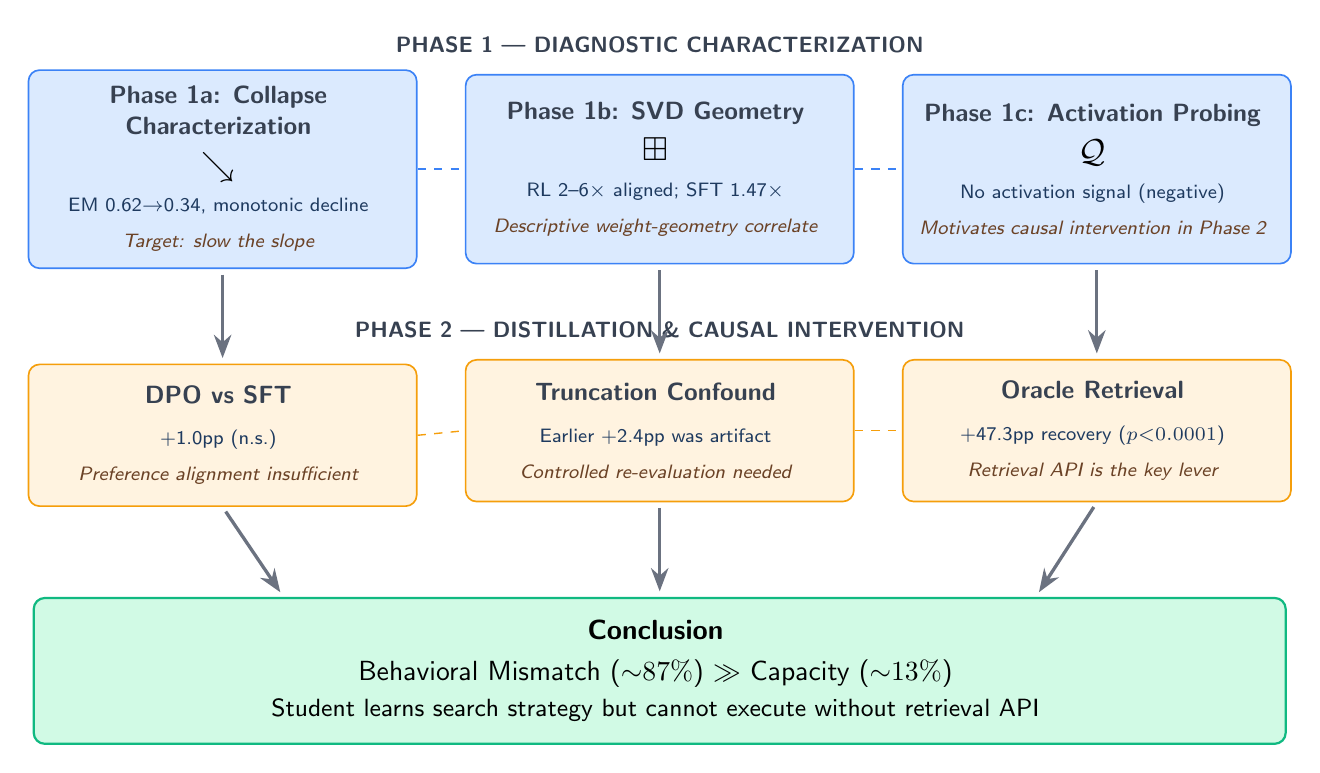
\begin{tikzpicture}[
    >=Stealth,
    every node/.style={font=\small\sffamily},
    p1box/.style={
        draw=phase1border, fill=phase1bg, rounded corners=4pt,
        minimum width=4.9cm, minimum height=2.4cm,
        inner sep=6pt, align=center,
        line width=0.6pt
    },
    p2box/.style={
        draw=phase2border, fill=phase2bg, rounded corners=4pt,
        minimum width=4.9cm, minimum height=1.8cm,
        inner sep=6pt, align=center,
        line width=0.6pt
    },
    concbox/.style={
        draw=concborder, fill=concbg, rounded corners=4pt,
        minimum width=15.9cm, minimum height=1.4cm,
        inner sep=8pt, align=center,
        line width=0.8pt
    },
    phaselabel/.style={
        font=\footnotesize\sffamily\bfseries, color=labelgray
    },
    phasearrow/.style={
        ->, arrowgray, line width=1.2pt,
        shorten >=2pt, shorten <=2pt
    },
]

% ===== Phase 1 boxes =====
\node[p1box] (p1a) {%
    \begin{minipage}{4.4cm}\centering
    {\small\sffamily\bfseries\color{labelgray} Phase 1a: Collapse Characterization}\\[4pt]
    {\large$\searrow$}\\[2pt]
    {\scriptsize\color{findingcolor} EM 0.62$\to$0.34, monotonic decline}\\[2pt]
    {\scriptsize\itshape\color{implcolor} Target: slow the slope}
    \end{minipage}
};

\node[p1box, right=0.6cm of p1a] (p1b) {%
    \begin{minipage}{4.4cm}\centering
    {\small\sffamily\bfseries\color{labelgray} Phase 1b: SVD Geometry}\\[4pt]
    {\large$\boxplus$}\\[2pt]
    {\scriptsize\color{findingcolor} RL 2--6$\times$ aligned; SFT 1.47$\times$}\\[2pt]
    {\scriptsize\itshape\color{implcolor} Descriptive weight-geometry correlate}
    \end{minipage}
};

\node[p1box, right=0.6cm of p1b] (p1c) {%
    \begin{minipage}{4.4cm}\centering
    {\small\sffamily\bfseries\color{labelgray} Phase 1c: Activation Probing}\\[4pt]
    {\large$\mathcal{Q}$}\\[2pt]
    {\scriptsize\color{findingcolor} No activation signal (negative)}\\[2pt]
    {\scriptsize\itshape\color{implcolor} Motivates causal intervention in Phase 2}
    \end{minipage}
};

% Phase 1 group label
\node[phaselabel, above=0.15cm of p1b] (p1label) {PHASE 1 --- DIAGNOSTIC CHARACTERIZATION};

% ===== Phase 2 boxes =====
\node[p2box, below=1.2cm of p1a] (p2a) {%
    \begin{minipage}{4.4cm}\centering
    {\small\sffamily\bfseries\color{labelgray} DPO vs SFT}\\[4pt]
    {\scriptsize\color{findingcolor} +1.0pp (n.s.)}\\[2pt]
    {\scriptsize\itshape\color{implcolor} Preference alignment insufficient}
    \end{minipage}
};

\node[p2box, below=1.2cm of p1b] (p2b) {%
    \begin{minipage}{4.4cm}\centering
    {\small\sffamily\bfseries\color{labelgray} Truncation Confound}\\[4pt]
    {\scriptsize\color{findingcolor} Earlier +2.4pp was artifact}\\[2pt]
    {\scriptsize\itshape\color{implcolor} Controlled re-evaluation needed}
    \end{minipage}
};

\node[p2box, below=1.2cm of p1c] (p2c) {%
    \begin{minipage}{4.4cm}\centering
    {\small\sffamily\bfseries\color{labelgray} Oracle Retrieval}\\[4pt]
    {\scriptsize\color{findingcolor} +47.3pp recovery ($p{<}0.0001$)}\\[2pt]
    {\scriptsize\itshape\color{implcolor} Retrieval API is the key lever}
    \end{minipage}
};

% Phase 2 group label
\node[phaselabel, above=0.15cm of p2b] (p2label) {PHASE 2 --- DISTILLATION \& CAUSAL INTERVENTION};

% ===== Conclusion box =====
\node[concbox, below=1.2cm of p2b] (conc) {%
    \begin{minipage}{14.8cm}\centering
    {\sffamily\bfseries\normalsize Conclusion}\\[4pt]
    {\normalsize Behavioral Mismatch (${\sim}87\%$) $\gg$ Capacity (${\sim}13\%$)}\\[2pt]
    {\small Student learns search strategy but cannot execute without retrieval API}
    \end{minipage}
};

% ===== Arrows: Phase 1 -> Phase 2 =====
\draw[phasearrow] (p1a.south) -- (p2a.north);
\draw[phasearrow] (p1b.south) -- (p2b.north);
\draw[phasearrow] (p1c.south) -- (p2c.north);

% ===== Arrows: Phase 2 -> Conclusion =====
\draw[phasearrow] (p2a.south) -- ($(conc.north west)!0.2!(conc.north east)$);
\draw[phasearrow] (p2b.south) -- (conc.north);
\draw[phasearrow] (p2c.south) -- ($(conc.north west)!0.8!(conc.north east)$);

% ===== Horizontal connectors in Phase 1 =====
\draw[-, phase1border, line width=0.5pt, dashed] (p1a.east) -- (p1b.west);
\draw[-, phase1border, line width=0.5pt, dashed] (p1b.east) -- (p1c.west);

% ===== Horizontal connectors in Phase 2 =====
\draw[-, phase2border, line width=0.5pt, dashed] (p2a.east) -- (p2b.west);
\draw[-, phase2border, line width=0.5pt, dashed] (p2b.east) -- (p2c.west);

\end{tikzpicture}
\end{document}
